% This is samplepaper.tex, a sample chapter demonstrating the
% LLNCS macro package for Springer Computer Science proceedings;
% Version 2.21 of 2022/01/12
%
\RequirePackage{amsmath}
\documentclass[runningheads]{llncs}

%
\usepackage[T1]{fontenc}
% T1 fonts will be used to generate the final print and online PDFs,
% so please use T1 fonts in your manuscript whenever possible.
% Other font encondings may result in incorrect characters.
%
\usepackage{graphicx}
% Used for displaying a sample figure. If possible, figure files should
% be included in EPS format.
%
% If you use the hyperref package, please uncomment the following two lines
% to display URLs in blue roman font according to Springer's eBook style:
%\usepackage{color}
%\renewcommand\UrlFont{\color{blue}\rmfamily}
%\urlstyle{rm}
%

\usepackage{comment}
\usepackage{tabularx}
\usepackage{todonotes} 

\usepackage{listings} 
\lstset{
  basicstyle=\footnotesize\tt,        % the size of the fonts that are used for the code
  breakatwhitespace=false,         % sets if automatic breaks should only happen at whitespace
  breaklines=true,                 % sets automatic line breaking
  captionpos=b,                    % sets the caption-position to bottom
  extendedchars=true,              % lets you use non-ASCII characters; for 8-bits encodings only, does not work with UTF-8
  frame=single,                    % adds a frame around the code
  language=Java,                 % the language of the code
  keywordstyle=\bf,
  showspaces=false,                % show spaces everywhere adding particular underscores; it overrides 'showstringspaces'
  showstringspaces=false,          % underline spaces within strings only
  showtabs=false,                  % show tabs within strings adding particular underscores
  tabsize=2                       % sets default tabsize to 2 spaces
}

% for subfigure
% warning ist ein bekanntes Problem
\usepackage{subcaption}

\usepackage{comment}


\newcommand{\patternname}[1]{\newpage{\large{\textsc{#1}}}}

\newcommand{\patternnameinline}[1]{\textsc{#1}}


%\textbf{\textsc{Foo}}

\newcommand{\patternOne}{
    \patternname{Pattern 1: Core of Content}
}

\newcommand{\patternTwo}{
    \patternname{Pattern 2: Accessibility of Diagrams}
}

\newcommand{\patternThree}{
    \patternname{Pattern 3: Accessibility of Graphics}
}

\newcommand{\patternFour}{
    \patternname{Pattern 4: Sonification of Time Series}
}

\newcommand{\patternFive}{
    \patternname{Pattern 5: Graphics with Generated Explanation}
}

\newcommand{\patternSix}{
    \patternname{Pattern 6: Accessibility-Aware AI Tutor}
}

\newcommand{\patternSeven}{
    % KI: C.10 benennt Pattern 7 um; der neue Name betont die strukturierte Begleitfunktion statt generischer Podcast-Erzeugung.
    \patternname{Pattern 7: Structured Audio Companion}

}

\newcommand{\patternOneInline}{
    \patternnameinline{Core of Content}
}

\newcommand{\patternTwoInline}{
    \patternnameinline{Accessibility of Diagrams}
}

\newcommand{\patternThreeInline}{
    \patternnameinline{Accessibility of Graphics}
}

\newcommand{\patternFourInline}{
    \patternnameinline{Sonification of Time Series}
}

\newcommand{\patternFiveInline}{
    \patternnameinline{Graphics with Generated Explanation}
}

\newcommand{\patternSixInline}{
    \patternnameinline{Accessibility-Aware AI Tutor}
}

\newcommand{\patternSevenInline}{
    % KI: C.10 hält die Inline-Bezeichnung konsistent zum neuen Pattern-Namen.
    \patternnameinline{Structured Audio Companion}
}

%\setlength\parindent{0pt}
%\usepackage{parskip}
\sloppy

\usepackage[nohyperlinks, printonlyused]{acronym}
% Acronym definitions used throughout the paper.
% Keep these definitions before the first \ac{...} usage.

\acrodef{ai}[AI]{artificial intelligence}
\acrodef{adhd}[ADHD]{attention-deficit/hyperactivity disorder}
\acrodef{csv}[CSV]{comma-separated values}
\acrodef{esa}[ESA]{European Space Agency}
\acrodef{gpt}[GPT]{generative pretrained transformer}
\acrodef{llm}[LLM]{large language model}
\acrodef{lms}[LMS]{learning management system}
\acrodef{mllm}[MLLM]{multimodal large language model}
\acrodef{nasa}[NASA]{National Aeronautics and Space Administration}
\acrodef{pdf}[PDF]{portable document format}
\acrodef{svg}[SVG]{Scalable Vector Graphics}
\acrodef{wai}[WAI]{Web Accessibility Initiative}
\acrodef{wcag}[WCAG]{Web Content Accessibility Guidelines}
\acrodef{bvi}[BVI]{blind and visually impaired}
\acrodef{gai}[GenAI]{generative artificial intelligence}
\acrodef{mds}[MDS]{Multimodal Diagrammatic System}
\acrodef{html}[HTML]{Hypertext Markup Language}
\acrodef{kv}[KV]{Karnaugh--Veitch}
\acrodef{mit}[MIT]{Massachusetts Institute of Technology}
\acrodef{oop}[OOP]{Object-Oriented Programming}
\acrodef{spice}[SPICE]{Simulation Program with Integrated Circuit Emphasis}
\acrodef{stem}[STEM]{Science, Technology, Engineering, and Mathematics}
\acrodef{tml}[TML]{textual modeling language}
\acrodef{uml}[UML]{Unified Modeling Language}
\acrodef{uncrpd}[UN-CRPD]{United Nations Convention on the Rights of Persons with Disabilities}
\acrodef{who}[WHO]{World Health Organization}
\acrodef{wysiwyg}[WYSIWYG]{What You See Is What You Get}
\acrodef{xml}[XML]{Extensible Markup Language}
\acrodef{xmi}[XMI]{XML Metadata Interchange}
\acrodef{yaml}[YAML]{Yet Another Markup Language}


\usepackage{xcolor}

\newenvironment{sol}
    {
    %\begin{itshape}
    \begin{bfseries}
    }
    { 
    \end{bfseries}
    \newline
    %\end{itshape}
    }
%

\usepackage[framemethod=TikZ]{mdframed}

\newenvironment{quoted}
    {
    %\begin{itshape}
    }
    { 
    %\end{itshape}
    }
%

\surroundwithmdframed[
    innertopmargin=4pt,
    innerbottommargin=4pt,
    innerrightmargin=4pt,
    innerleftmargin=4pt
]{quoted}

\usepackage{hyperref}
\hypersetup{
    colorlinks=true,
    linkcolor=blue,
    filecolor=magenta,      
    urlcolor=cyan,
    pdftitle={A Pattern Collection for Generating Accessible Teaching Materials in STEM},
    pdfpagemode=FullScreen,
}

% Auswahl der included sections, geht nicht, weil Seitenzahl dann springt
%\includeonly{title_abstract, introduction, 6_Pattern, 7_Pattern, Conclusion_and_Future_Work}


\begin{document}

\title{A Pattern Collection for Generating Accessible Teaching Materials  in \ac{stem}}

\titlerunning{Accessible Teaching Materials in \ac{stem}}

\author{Diethelm Bienhaus\inst{1}\orcidID{0000-0002-9207-3412}  
\and \\
Michael Kreutzer\inst{1}\orcidID{0000-0003-0748-7707}
\and \\
Florian von Zabiensky\inst{1}\orcidID{0000-0003-0951-0288}}
%
\authorrunning{D. Bienhaus, M. Kreutzer, F. v. Zabiensky}



\institute{Technische Hochschule Mittelhessen University of Applied Sciences, Germany
\email{\{diethelm.bienhaus, michael.kreutzer\}@mni.thm.de},
\\
Website: \url{mni.thm.de}
}
%
\maketitle              % typeset the header of the contribution
%

\begin{abstract}
\ac{stem} education relies heavily on visual artifacts such as diagrams, circuit schematics, plots, tables, formulas, and graphical simulation tools. These artifacts often remain difficult or impossible to access for \ac{bvi} students when they are only provided as visual representations. At the same time, long and densely structured academic materials can impose additional barriers for learners with impairments such as \ac{adhd} or dyslexia, who may benefit from segmented and multimodal access.

This paper extends the EuroPLoP 2025 pattern collection \textit{A Pattern Collection for Generating Accessible Teaching Materials for Blind and Visually Impaired Students in Computer Science and Electrical Engineering}. The earlier collection focused on transforming visual \ac{stem} artifacts into accessible textual, tactile, or auditory representations. We add two AI-mediated patterns that address accessibility during actual learning situations rather than only during material preparation.

\textsc{Accessibility-Aware AI Tutor} describes how to provide persistent, course-specific, and accessibility-aware support that is grounded in curated course materials, explicit accessibility rules, and repeatable transformation workflows. \textsc{Structured Audio Companion} describes how to provide segmented, source-grounded audio orientation with transcripts, timecodes, and explicit pointers to precise accessible representations of visual artifacts.

Together, the two patterns show that generative artificial intelligence can support accessibility when it is embedded in course context, stable workflows, and human-in-the-loop quality assurance. AI-generated explanations and audio summaries should not replace precise accessible representations of visual \ac{stem} artifacts; rather, they should help learners find, understand, and use them.

\keywords{Accessibility \and Blind and Visually Impaired Learners \and STEM Education \and Generative Artificial Intelligence \and Large Language Models \and ADHD \and Dyslexia}
\end{abstract}

% Keywords: Accessibility, Blind and Visually impaired Learners, Large Language Models,  Attention-Deficit/Hyperactivity Disorder (ADHD), Dyslexia

\section{Introduction}

Germany continues to face a substantial shortage of workers in Science, Technology, Engineering, and Mathematics (STEM). According to the MINT-Herbstreport 2025, the aggregated STEM labour shortage amounted to 148,500 workers in October 2025, including 40,800 in academic STEM expert occupations \cite{Anger2025MINT}.

Science, Technology, Engineering, and Mathematics (STEM) disciplines offer favorable study and career prospects, also for people with disabilities. These fields place a strong emphasis on technical competencies and are characterized by highly structured content, which can be advantageous for diverse learning needs. Moreover, assistive technologies such as screen readers, speech recognition and output systems, as well as adapted workplace design and flexible work organization enable many people with disabilities to participate effectively in STEM education and employment.

Nevertheless, students with disabilities continue to encounter substantial barriers during their studies. These barriers arise from both structural and organizational conditions within higher education. Technical obstacles include limited accessibility of learning materials, especially those that rely heavily on visual representations or the use of complex graphical software tools. In addition, learning environments that are overly complex, poorly structured, or highly nested can impose a significant cognitive load on students with impairments such as attention-deficit/hyperactivity disorder, autism spectrum conditions, depression, or chronic fatigue.

As a result, learning progress may be slowed for students with disabilities, despite adequate or even high professional qualifications. Importantly, however, many of these barriers can be mitigated through relatively small and targeted measures that substantially improve accessibility. The patterns presented in this paper therefore aim to address key problems and challenges relevant to inclusive learning in STEM education.

\section{The Pattern Collection}

The pattern collection "A Pattern Collection for Generating Accessible Teaching Materials for Blind and Visually Impaired Students in Computer Science and Electrical Engineering" presented at EuroPLoP 2025 comprises five patterns:

\patternOneInline provides a general approach for gaining accessibility for \ac{bvi} students. 
The two patterns \patternTwoInline and \patternThreeInline introduce specialized solutions for different types of graphically represented teaching content. 
\patternFiveInline can be applied to gain accessibility of different types of graphics. 
\patternFourInline shows how time series can be made audible and thus accessible to \ac{bvi} people.

\newpage
\subsection*{Overview of the Pattern Collection from 2025}
\vspace{-2em}
%%%%%%%%%%%%%%%%% 1 1%%%%%%%%%%%%%%%%%%%%%%%%%%%%%%%%%
\begin{table}[!ht]
    \centering
    \begin{tabularx}{\textwidth}{|p{0.12\textwidth}|X|}
    \hline
         Pattern 1 &  \textsc{Core of Content}  \\ \hline
         Problem & Graphics are usually not accessible for the visually impaired.  Text within graphics cannot be extracted by assistive tools.  \\ \hline
         Solution & Extract the core content of teaching materials and represent it in a multi-directionally transformable format.  \\ \hline
    \end{tabularx}
\end{table}
\vspace{-3em}
%%%%%%%%%%%%%%%%% 2 %%%%%%%%%%%%%%%%%%%%%%%%%%%%%%%%%
\begin{table}[!ht]
    \centering
\begin{tabularx}{\textwidth}{|p{0.12\textwidth}|X|}
    \hline
         Pattern 2 & \textsc{Accessibility of Diagrams}  \\ \hline
         Problem &  Graphical representations of diagrams are not accessible to \ac{bvi} learners. \\ \hline
         Solution &  Analyze which concepts are represented by the diagram and find a textual representation for them. 
Implicit information as expressed by the spatial arrangement of diagram elements can be made tangible with haptic interface devices.  \\ \hline
\end{tabularx}
\end{table}
\vspace{-3em}
%%%%%%%%%%%%%%%%% 3 %%%%%%%%%%%%%%%%%%%%%%%%%%%%%%%%%
\begin{table}[!ht]
    \centering
\begin{tabularx}{\textwidth}{|p{0.12\textwidth}|X|}
    \hline
         Pattern  3 & \textsc{Accessibility of Graphics}  \\ \hline
         Problem &  Non-textual content—such as images, maps, charts, and diagrams remains largely inaccessible to \ac{bvi} students. This inaccessibility presents a significant barrier to information acquisition and equal participation in educational and professional environments.  \\ \hline
         Solution &  Provide textual, tactile, or auditory access to information represented visually in graphics.  \\ \hline
\end{tabularx}
\end{table}
\vspace{-3em}
%%%%%%%%%%%%%%%%% 4 %%%%%%%%%%%%%%%%%%%%%%%%%%%%%%%%%
\begin{table}[!ht]
    \centering
\begin{tabularx}{\textwidth}{|p{0.12\textwidth}|X|}
    \hline
         Pattern 4 & \textsc{Sonification of Time Series}  \\ \hline
         Problem & Graphical representations of time series  are not accessible for \ac{bvi} students and people in general. A sequential output of the data on Braille lines or by means of text-to-speech is not well suited to represent and convey the time based aspect of the data.   \\ \hline
         Solution &  Provide sonifications of time series. \\ \hline
\end{tabularx}
\end{table}
\vspace{-3em}
%%%%%%%%%%%%%%%%% 5 %%%%%%%%%%%%%%%%%%%%%%%%%%%%%%%%%
\begin{table}[!ht]
    \centering
\begin{tabularx}{\textwidth}{|p{0.12\textwidth}|X|}
    \hline
         Pattern 5 & \textsc{Graphics with Generated Explanation}  \\ \hline
         Problem &  Although electronic media can be made accessible to \ac{bvi} learners through the use of assistive technologies, this does not usually work for the graphic components embedded in these media. \\ \hline
         Solution &  Augment visually represented information with a generated and verified textual description.  \\ \hline
\end{tabularx}
\end{table}

This collection is extended by two additional patterns, \patternSixInline and \patternSevenInline. Figure~\ref{fig:pattern-relationships} shows Pattern~1 as the foundation of the collection. Patterns~2 to~5 provide specialized transformations of visual \ac{stem} artifacts. Pattern~6 uses and orchestrates these transformations in interactive learning situations, while Pattern~7 provides an audio-oriented overview and points learners to precise accessible representations where needed.

% KI: Robuste tabularx-Figur statt TikZ: kompiliert mit vorhandenen Paketen und bleibt vollständig editierbar.
\begin{figure}[ht]
\centering
\small
\setlength{\tabcolsep}{4pt}
\renewcommand{\arraystretch}{1.25}
\begin{tabularx}{\textwidth}{|p{0.18\textwidth}|X|}
\hline
\textbf{Layer 1: Foundation} & \textbf{Pattern 1: \textsc{Core of Content}} \\
\hline
\multicolumn{2}{|c|}{$\Downarrow$ foundation for all following patterns} \\
\hline
\textbf{Layer 2: Accessible representations} & \textbf{Patterns 2--5:} \textsc{Accessibility of Diagrams}; \textsc{Accessibility of Graphics}; \textsc{Sonification of Time Series}; \textsc{Graphics with Generated Explanation} \\
\hline
\textbf{Layer 3: AI-mediated support} & \textbf{Pattern 6: \textsc{Accessibility-Aware AI Tutor}} uses, orchestrates and explains Patterns 2--5 in interactive learning situations. \newline
\textbf{Pattern 7: \textsc{Structured Audio Companion}} summarizes and orients learners, and points to precise accessible representations where visual artifacts contain essential technical information. \\
\hline
\textbf{Verification relation} & Pattern 5 and Pattern 6 require verification and human-in-the-loop quality assurance when generated explanations are used. \\
\hline
\end{tabularx}
\caption{Pattern relationships in the extended collection. Pattern~1 provides the foundation. Patterns~2--5 provide specialized accessible representations for visual \ac{stem} artifacts. Pattern~6 uses these patterns for interactive AI-supported learning, while Pattern~7 offers audio-oriented orientation and points back to precise accessible representations.}
\label{fig:pattern-relationships}
\end{figure}


% KI: D.15 bindet Related Work zentral ein; pattern-spezifische Related-Work-Blöcke werden dadurch vermieden.
% KI: D.15 zentralisiert Related Work, damit die einzelnen Patterns nicht wie separate Mini-Papers wirken.
\section{Related Work}

\subsection{Accessible STEM representations and AI-supported visual explanations}

Recent work explores \ac{llm} and \ac{mllm} based tools as assistive technologies that translate visually encoded information into representations that can be perceived and navigated by \ac{bvi} users. Empirical evaluations indicate that \ac{mllm}s can support common visual assistance tasks, while reliability and error handling remain central challenges for broader use \cite{Karamolegkou2025}. Generative AI for accessible content production has recently gained significant attention as a promising strategy for reducing educational barriers. Research demonstrates that large language models and image-to-text systems can automatically generate alternative text, audio descriptions, or multi-modal summaries, thereby supporting blind and visually impaired learners in \ac{stem} and other fields \cite{Karamolegkou2025,Schauer2025}.

In the domain of data visualizations, conversational systems such as \textit{VizAbility} demonstrate how dialogue-based interaction can augment chart exploration \cite{Gorniak2024VizAbility}. Complementary work emphasizes that accessibility is not achieved by static descriptions alone but depends on interaction mechanisms that preserve user agency and enable independent exploration with screen readers \cite{Sharif2025VoxEx}.

A second line of related research focuses on making diagram semantics explicit so that users can query or learn from diagrams through language-based interaction. Approaches that generate detailed textual descriptions of diagrams for \ac{llm}-based exploration illustrate how ``silent'' graphics can be bridged into structured natural language, supporting accessible learning pathways for \ac{bvi} users \cite{Wegwerth2023Diagram}.

There is ongoing research how to extract circuit structure from schematics and generating netlists automatically. \cite{Hemker2024Schematics,Huang2025Netlistify} present deep-learning-based schematic-to-netlist pipelines demonstrating progress in component recognition and connectivity extraction.

For time-dependent simulation outputs, related state-of-the-art work on sonification and haptic feedback provides additional non-visual access that can complement text-based traces and key metrics \cite{Spagnuolo2025Sonification}.

\subsection{Audio summaries and multimodal learning support}

Structured educational podcasts have been studied as an accessible learning modality for \ac{bvi} users, showing that clear structure and navigability matter \cite{Buzzi2011StructuredPodcasts}. Speech-first summarization research emphasizes that summaries optimized for spoken output require different design choices than text summaries and should explicitly support linear comprehension \cite{McKeown2005TextToSpeech}.

Recent accessibility research explores AI-assisted navigation and question answering to help \ac{bvi} learners access lecture content more efficiently \cite{Anderer2025LectureVideos}, aligning with our goal of reducing first-pass overhead for large material bundles. Recent studies of AI-generated educational podcasts report positive learner experiences and measurable learning outcomes in educational settings \cite{Do2024PAIGE}. Podcast-like course materials should be supplemented with textual information to enable targeted access to the audio information and to provide alternative channels.

% KI: Ergänzt eine konzeptionelle Brücke zwischen Related Work und den beiden neuen AI-Patterns.
% KI: Diese Section ergänzt eine konzeptionelle Übersicht über die AI-vermittelte Erweiterung der Pattern Collection.
\section{AI-mediated Extension of the Pattern Collection}

Figure~\ref{fig:ai-workflow} summarizes how the two new patterns are applied in relation to course materials. Course materials such as slides, scripts, exercises, figures, and simulation outputs are first prepared in a curation layer. This layer contains course context, terminology, learning goals, accessibility rules, and transformation workflows. Pattern~6 then provides interactive accessible outputs such as explanations, diagram descriptions, netlists, tables, and quality-assurance prompts. Pattern~7 provides audio-oriented outputs such as segmented audio overviews, transcripts, timecodes, and references to figures and tables. Both branches converge in accessible learning support: screen-reader-friendly explanations, precise representations, orientation and review, and human-in-the-loop quality assurance.

% KI: Robuste tabularx-Figur statt TikZ: kompiliert mit vorhandenen Paketen und bleibt vollständig editierbar.
\begin{figure}[ht]
\centering
\small
\setlength{\tabcolsep}{4pt}
\renewcommand{\arraystretch}{1.25}
\begin{tabularx}{\textwidth}{|X|}
\hline
\textbf{Course Materials} \\
slides, scripts, exercises, figures, simulations \\
\hline
\multicolumn{1}{c}{$\Downarrow$} \\
\hline
\textbf{Curation Layer} \\
course context; terminology; learning goals; accessibility rules; transformation workflows \\
\hline
\multicolumn{1}{c}{$\Downarrow$} \\
\hline
\begin{tabularx}{\textwidth}{X@{\hspace{0.05\textwidth}}X}
\textbf{Pattern 6: Accessibility-Aware AI Tutor} & \textbf{Pattern 7: Structured Audio Companion} \\
interactive explanations; diagram descriptions; netlists; tables; QA prompts & segmented audio overview; transcript; timecodes; references to figures and tables \\
\end{tabularx} \\
\hline
\multicolumn{1}{c}{$\Downarrow$} \\
\hline
\textbf{Accessible Learning Support} \\
screen-reader-friendly explanations; precise representations; orientation and review; human-in-the-loop quality assurance \\
\hline
\end{tabularx}
\caption{AI-mediated accessibility workflow. AI is embedded in explicit workflows, curated course context, and quality assurance. Pattern~6 produces interactive accessible outputs, while Pattern~7 provides structured audio orientation. Audio supports orientation; it does not replace precise accessible representations.}
\label{fig:ai-workflow}
\end{figure}


%\patternname{Pattern Template}

\subsection*{Context}
	
    
\subsection*{Problem}


\subsection*{Solution}



\subsection*{Examples}
 
\subsection*{Consequences}

% Benefits
\renewcommand{\labelenumi}{$+$}
\begin{enumerate}
\item Lorem ipsum dolor sit amet, consetetur sadipscing elitr, sed diam nonumy eirmod tempor invidunt ut labore et dolore magna aliquyam
\item Lorem ipsum dolor sit amet, consetetur sadipscing elitr, sed diam nonumy eirmod tempor invidunt ut labore et dolore magna aliquyam
\item Lorem ipsum dolor sit amet, consetetur sadipscing elitr, sed diam nonumy eirmod tempor invidunt ut labore et dolore magna aliquyam
\end{enumerate}

% Liabilities
\renewcommand{\labelenumi}{$-$}
\begin{enumerate}
\item Lorem ipsum dolor sit amet, consetetur sadipscing elitr, sed diam nonumy eirmod tempor invidunt ut labore et dolore magna aliquyam
\item Lorem ipsum dolor sit amet, consetetur sadipscing elitr, sed diam nonumy eirmod tempor invidunt ut labore et dolore magna aliquyam
\item Lorem ipsum dolor sit amet, consetetur sadipscing elitr, sed diam nonumy eirmod tempor invidunt ut labore et dolore magna aliquyam
\end{enumerate}
 
\subsection*{Related Work}
	
     % Template / Testen

%\patternOne

\subsection*{Context}

Visually appealing course materials are a goal for many educators and are appreciated by students. 

Graphically designed course materials are appealing for sighted people. Graphics support the content to be taught. 

\ac{wysiwyg} tools such as Word or PowerPoint make it very easy to place graphics almost anywhere. 

\subsection*{Problem}

\begin{itshape}

Graphics are usually not accessible for the visually impaired. 
Text within graphics cannot be extracted by assistive tools.

\end{itshape}
    
    



\subsection*{Solution}

\begin{sol}
Extract the core content of teaching materials and represent it in a multi-directionally transformable format.
\end{sol}


First, eliminate all purely decorative graphics.
Analyze whether and what information is conveyed by typographic layout. 
Identify the graphics that carry the content to be taught.


This paper distinguishes between diagrams and graphics. 
In case of diagrams that adhere to a formal specification, such specifications typically define formats for textual representation. These structured formats enable systematic interpretation, transformation, and accessibility enhancement through computational means. 
Pattern \patternTwoInline presents solutions to gain accessibility for this type of diagrams. 

By contrast, graphics such as photographs, freehand drawings, and various other illustrative visualizations do not follow a formal specification. As a result, there is no underlying metamodel that can be leveraged to interpret or describe their content programmatically.
To make such unstructured graphics accessible—particularly for \ac{bvi} students haptic solutions are a promising approach. Tactile representations provide a means of conveying the structural and spatial properties of these graphics in a non-visual form, as introduced in pattern \patternThreeInline. 
 
Use simple, plain-text formats with minimal formatting whenever possible.
Plain text is easy to process with screen readers, Braille displays, and text-to-speech tools, making it more accessible for \ac{bvi} students. Markdown is a particularly suitable format. It offers basic yet effective formatting options and can be easily converted into various output formats such as HTML or PDF. However, purely textual materials may not be engaging for sighted students. They are accustomed to visually rich course materials, such as textbooks, handouts, and slide decks that follow well-designed layouts.
To address this, rendering tools can be used to convert the core content into visually appealing formats. By generating PDFs or web-based HTML documents, course materials can be presented in a way that meets the expectations of sighted learners—without compromising accessibility.

\subsection*{Examples}
 
Fig.~\ref{fig:questionmark} shows an example of a graphic that is used only for decoration. Such graphics do not carry any content. If they are to be used for visual reasons, the graphic should be labeled as purely decorative in the text-only version of the course materials.

\begin{figure}
    \centering
    \fbox{\includegraphics[page=3, width=0.12\linewidth]{img/out.pdf}}
    \caption{Solely decorative image}
    \label{fig:questionmark}
\end{figure}



Fig.~\ref{fig:freehand} shows an example where two small pictures are freely positioned on a slide. They illustrate the explanatory text left of them. However, they contribute to the content. Arrows point to the words "Dog" and "Human". The arrows shall visualize the  relationships "generalization" and "specialization" between classes in object-oriented programming. 

\begin{figure}[ht!]
    \centering
    \fbox{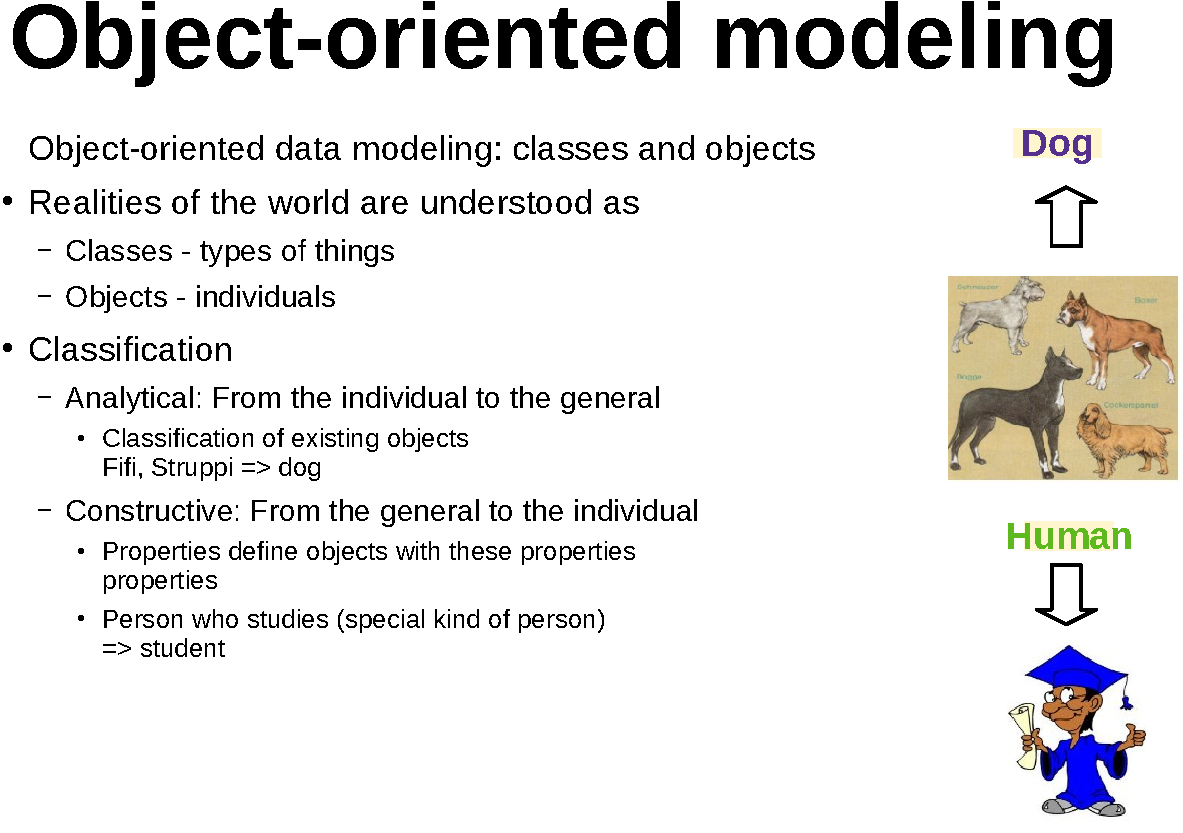
\includegraphics[page=1, width=0.7\linewidth]{img/out.pdf}}
    \caption{Pictures and tool-accessible text placed freehand on a slide}
    \label{fig:freehand}
\end{figure}

The words "Dog" and "Human" can be found by assisting tools. The arrows and the content of the small pictures are not accessible. 
Intended was an additional visualization of the concepts which are described in the text on the left side. It would be better to use diagrams whose structure is specified and which can be represented textually as introduced in the pattern \patternTwoInline.




The author of the following slide (Fig.~\ref{fig:table}) has inserted a table as an image on the slide. Arrows point to areas of the image and link explanations to the actual elements of the table.




\begin{figure}[ht!]
    \centering
    \fbox{\includegraphics[page=2, width= \linewidth]{img/out.pdf}}
    \caption{Table included as an image and mixed with textual information on a slide (image source: www.onlinemathlearning.com/)}
    \label{fig:table}
\end{figure}

The table is not accessible for the visually impaired. Explanations are extracted as text by assistive systems. The assignments and the table cannot be extracted. It is better to insert the table as a textual table. 
Explanations should also be assigned to the contents of the table as text.


Markdown is designed to use a minimal set of tags. Hence, it is easier to parse when access is done via text-to-speech or is read on a Braille display. 
Tools like Pandoc\footnote{\url{https://pandoc.org/}} can convert markdown text in a variety of formats like PDF, \ac{html} and office formats. As a result, it is possible to provide the clean text with the content for \ac{bvi} students and to give the others rendered outputs (e.g., PDF).

\newpage
Listing \ref{lst:table} shows the Markdown text which is rendered into the slide shown in Fig.~\ref{fig:table} using Pandoc.  


\begin{lstlisting}[label = lst:table, caption = Markdown of the slide in Fig~\ref{fig:table}]
# Boolean Operations
Operation: Conjunction
Operation name: AND
Input Variables: P, Q
Operation formula: $P \land Q$ 

Truth table:
| P | Q | P AND Q |
|---|---|-----|
| 0 | 0 | 0   |
| 0 | 1 | 0   |
| 1 | 0 | 0   |
| 1 | 1 | 1   |
\end{lstlisting}


This markdown is then converted into a slide in PDF using Pandoc with a user defined \LaTeX Beamer template accomplishing the CI specifications of the university.
\begin{figure}
    \centering
    \fbox{\includegraphics[page=2, width=0.8\linewidth]{img/Slides_Template.pdf}
    }
    \caption{Slide generated from markdown text}
    \label{fig:slideexample}
\end{figure}

The slides have the usual layout for sighted students.  
The markdown text is provided for the visually impaired and is easily accessible for them using assistive technologies. 


\subsection*{Consequences}



% Benefits
\renewcommand{\labelenumi}{$+$}
\begin{enumerate}
   \item Textual descriptions of graphics make them accessible for \ac{bvi} learners
\item Various output channels such as Braille displays or text-to-speech can be used by \ac{bvi} learners
\item Authors are encouraged to focus on the core content of the teaching materials
\item pure text based representations are independent from proprietary office tools and incompatibility problems can be avoided 
 
\end{enumerate}

% Liabilities
\renewcommand{\labelenumi}{$-$}
\begin{enumerate}
\item The creation of teaching materials takes longer
    \item Tool chains must be set up to generate teaching materials for sighted people
\item Changes and corrections are more time-consuming during creation because the tool chain for generating teaching materials for sighted people must be triggered again and again
\item Free manual placement of graphics on slides and other teaching materials is not possible
    \item Inserting content such as tables as screen shots from textbooks or websites should be avoided, but this leads to more work because the content has to be rewritten in text form
\item Graphic design options such as placing arrows over graphics to visualize relationships are limited
\end{enumerate}
 
\subsection*{Related Work}

Prior research has demonstrated that single-source authoring can enable
accessible learning materials for \ac{bvi} students in STEM.
The \emph{PreTeXt} project illustrates how semantically structured source files
can be transformed into multiple accessible outputs, including web, EPUB, and
Braille, while maintaining consistency across modalities
\cite{Austin2024PreTeXt}. 

Complementary studies on lightweight markup (e.g., R
Markdown) show that such workflows reduce authoring overhead and generate
accessible HTML and PDF outputs that integrate well with screen readers
\cite{Seo2019RMarkdown}. 

For mathematical content, web-based outputs can rely
on MathJax together with the Speech Rule Engine to provide adaptable
accessibility features such as structural navigation and speech rendering,
making them effective for non-visual exploration
\cite{CervoneSorge2019W4A}. 

When PDF is required, \LaTeX-based tool chains can
embed tagged formulae to improve screen-reader access; however, these retrofits
remain more fragile than web-first alternatives
\cite{Armano2018LaTeXPDF}.



%\patternTwo

\subsection*{Context}

    Diagrams are an important form of representation, especially in technical disciplines. They are used for communication between people and for documentation. 
Such diagrams are usually precisely specified. 

In computer science, \ac{uml} diagrams  are widely used. There are specifications for \ac{uml}. Formats are defined for the data exchange of \ac{uml} models. 
Some software tools support code generation or reverse engineering.

In the first two semesters, it is mainly class diagrams that are taught.

Class diagrams primarily show the elements within classes and the relationships between classes as two-dimensional visual graphics.
    
\subsection*{Problem}

\begin{itshape}
Graphical representations of diagrams are not accessible to \ac{bvi} learners.
\end{itshape}

\subsection*{Solution}

\begin{sol}
Analyze which concepts are represented by the diagram and find a textual representation for them. 
Implicit information as expressed by the spatial arrangement of diagram elements can be made tangible with haptic interface devices.  
\end{sol}

Most software modeling tools use  a textual storage format. These formats are often not designed for humans but are used for data exchange. One example is \ac{xmi}\footnote{\url{https://www.omg.org/spec/XMI/}} for the exchange of \ac{uml} models. Model elements are represented textually as XML structures .

There are tools that use a simple textual representation that is easier for humans to read. UML4ALL, PlantUML and Mermaid are examples of such text based \ac{uml} tools.
These tools generate diagrams from the textual description for visual users. 
\ac{bvi} learners can have the textual description read aloud using text-to-speech, use screen readers or read on Braille lines.

A two-dimensional graphic is perceived by sighted people by “jumping” between the spatially arranged elements with the eye.
\ac{bvi} learners have sequential, one-dimensional access to the textual description. In order not to increase the cognitive load unnecessarily, information on relationships between elements should be provided near to the description of the elements.
The spatial arrangement of elements in a diagram often contains implicit information such as grouping or proximity of content. 
Such information can be made haptically accessible to \ac{bvi} learners. Examples include 2D Braille displays or structured surfaces (Swell Touch Paper, 3D printing).




\subsection*{Examples}
 
Listing \ref{lst:uml} is an example of a textual description following these recommendations and \ref{fig:class_diagram} shows the generated \ac{uml} class diagram. 


\begin{lstlisting}[label = lst:uml,  caption = {PlantUML source code}, basicstyle=\footnotesize]
@startuml
class Person {
  + firstname: String
  + surname: String
}
class Student {
  + matriculationNumber: int
  + degreeProgram: String
}
Person ^-- Student
class Lecturer {
  + title: String
  + department: String
}
Person ^-- Lecturer
class Book {
  + title: String
  + ISBN: String
}
Student "1" o-- "n" Book
@enduml
\end{lstlisting}

\begin{figure}[ht]
    \centering
    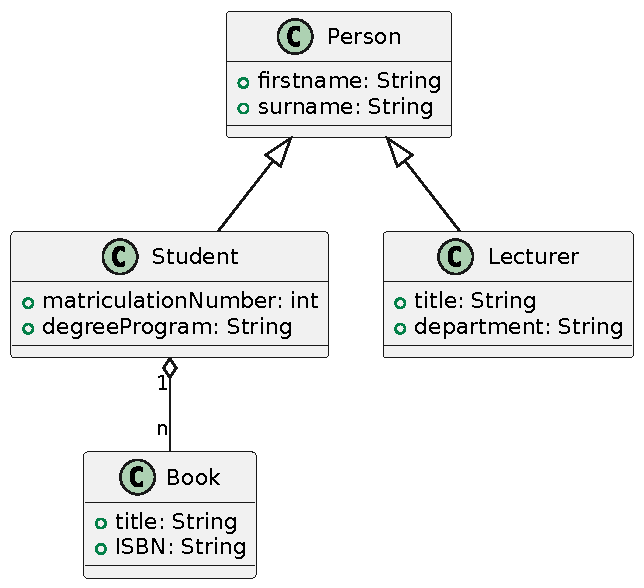
\includegraphics[width=.6\linewidth]{img/classDiagram.pdf}
    \caption{Generated \ac{uml} Class Diagram}
    \label{fig:class_diagram}
\end{figure}

\subsection*{Consequences}

% Benefits
\renewcommand{\labelenumi}{$+$}
\begin{enumerate}
\item Multi-modal accessibility is achieved by making textual explanations of diagrams accessible using assistive technology. 

\item Haptic devices can make information available that is contained in the spatial arrangement of elements in diagrams.

\item Textual descriptions of diagrams can be used in part to generate code. 
\end{enumerate}

% Liabilities
\renewcommand{\labelenumi}{$-$}
\begin{enumerate}
\item A new, purely text-based representation must be learned for the creation of teaching materials.

\item Changes and corrections are often more time-consuming, as the graphic representation must be re-rendered after changes are made.

\item Text-based exchange formats such as XMI are designed to be easily processed by software – but not primarily for human readability.
\end{enumerate} 
 
\subsection*{Related Work}

In \cite{doore2023} a \ac{mds} facilitates the perception of graphical information for \ac{bvi} students by integrating multiple sensory modalities: visual, auditory, and haptic. 
The system generates an auditory representation of diagrams by means of programmatically generated sine wave tones. Simultaneously, haptic feedback is delivered via a vibration motor, triggered when a user’s finger contacts specific x-y screen coordinates corresponding to points, lines, or curves. 

In \cite{king2007} the author present a project which makes  the content of UML diagrams accessible for \ac{bvi} students. In that project, a user interface for Windows was developed using the standard components of Microsoft Windows so that it is compatible with screen readers. This allows experienced users to use their usual screen reader. In addition, alternative interfaces such as spatial sound or a force feedback joystick are used to display spatial information on the diagram. 



In \cite{wildhaber2020} a solution is presented that allows visually impaired people easy access to class diagrams.
It utilizes existing accessibility tools of current mobile devices. A physically tactile grid is attached over a tablet so that a tactile navigation is possible.
By using Apple software, navigation can be carried out with the native VoiceOver solution, which is well known among  visually impaired people.
The authors developed a user interface which arranges classes in a grid.  Detailed information is displayed in a separate area, which can be navigated using the  VoiceOver system. 
In studies, the authors have compared their solution with the \ac{tml} PlantUML. Across several studies, the authors found that their solution is often better suited to new users, as it significantly lowers the learning curve compared to PlantUML.

%\patternThree

\subsection*{Context}

    Graphics constitute a fundamental modality of visual representation for sighted individuals. They are deeply integrated into everyday life, appearing in various forms such as city maps, architectural floor plans, and numerous types of instructional illustrations.

In educational contexts, graphical representations are extensively employed in teaching materials at both school and university levels. These include diagrams, sketches, and technical drawings, which are often created using software tools or produced as freehand illustrations.

    
\subsection*{Problem}

\begin{itshape}

However, non-textual content—such as images, maps, charts, and diagrams—remains largely inaccessible to \ac{bvi} students. This inaccessibility presents a significant barrier to information acquisition and equal participation in educational and professional environments.

\end{itshape}

\subsection*{Solution}

\begin{sol}

Provide textual, tactile, or auditory access to information represented visually in graphics.
  
\end{sol}

In HTML files the so called "alt text"  (alternative text) can give an additional text-based descriptions of visual details of an image. 
Originally intended to give some information if the HTML page is not loaded properly. 
Such descriptions are useful to provide accessible information for people who are visually impaired. This approach can be applied in other formats, too.


Important authoritative regulatory and guideline documents for "alt-text" are  W3C: "Web Content Accessibility Guidelines (WCAG)" \footnote{\url{https://www.w3.org/TR/WCAG21/}}, W3C WAI: “Resources on Alternative Text for Images” \footnote{\url{https://www.w3.org/WAI/alt/}}, W3C WAI: “Understanding Guideline 1.1: Text Alternatives” \footnote{\url{https://www.w3.org/WAI/WCAG22/Understanding/text-alternatives}}, and \ac{uncrpd}: "The Convention on the Rights of Persons with Disabilities"  \footnote{\url{https://social.desa.un.org/issues/disability/crpd/convention-on-the-rights-of-persons-with-disabilities-crpd}}


To make graphics perceivable through touch, they must be converted into raised, tangible structures. 
Color gradients present a significant challenge in this context. Instead, black-and-white graphics composed of lines, contours, and strokes are generally more suitable for tactile representation.

For more complex graphics that include areas beyond simple contours, the first step is to identify the edges of shapes. Many software tools begin this process by converting images into grayscale. Edge detection filters are then applied to extract outlines and essential details. Once the graphic is sufficiently simplified, it can be transformed into a tactile format using raised structures.

Additional information about a graphic can be embedded as metadata. Assistive technologies such as 2D Braille displays can then present this information as text or audio output.

Emerging \ac{ai} technologies are increasingly capable of interpreting and describing graphics. These advancements offer promising solutions for making visual content more accessible to \ac{bvi} students.

One solution for creating raised structures on paper is the use of Swell Touch Paper. This special paper can be printed on using standard printers or written on with a pen. When heat is applied, the printed areas expand, forming raised contours that are easily perceivable by touch.

3D printers have also gained popularity as a tool for producing tactile graphics. They allow for the creation of detailed contours and textures. Educational materials printed in this way are durable and can be reused over extended periods.

Electronic tactile displays, such as 2D Braille displays, provide dynamic tactile feedback. These devices can render static or even animated graphics in real time. They work by precisely raising and lowering an array of pins to create touchable images and patterns.



\subsection*{Examples}


An alternative text for Fig.~\ref{fig:class_diagram}
is generated using a web-site that supports generating alt-text by means of \ac{ai}\footnote{\url{https://barrierefreies.design/werkzeuge/ki-generator-alternativer-text-von-bildern}}.devices. The generated alt-text:
\begin{quoted}
   UML class diagram showing Person superclass with subclasses Student and Lecturer; Student linked to multiple Books with attributes like title and ISBN.
\end{quoted}

Class members were unfortunately suppressed by this tool.

Prompt for chatGPT: "write a alt-text for a html web site describing this diagram". Answer:
\begin{quoted}
UML class diagram showing four classes and their attributes. The classes are Person (attributes: firstname, surname), Student (matriculationNumber, degreeProgram), Lecturer (title, department), and Book (title, ISBN). Student and Lecturer both inherit from Person. There is an association from Person to Book indicating that one person can be linked to many books (1 to n).
\end{quoted}

This description contains the details of the class diagram. 


\textit{PunktBilder} is a software developed at the centre for blind persons (BliZ) at THM.
The \textit{PunktBilder} software is used to create tactile images for \ac{bvi} students at THM. Images are displayed in \textit{PunktBilder} (Fig.~\ref{fig:punktbilder}, ~\ref{fig:punktbilder2}) and can control  2D Braille displays. 

\begin{figure}
    \centering
    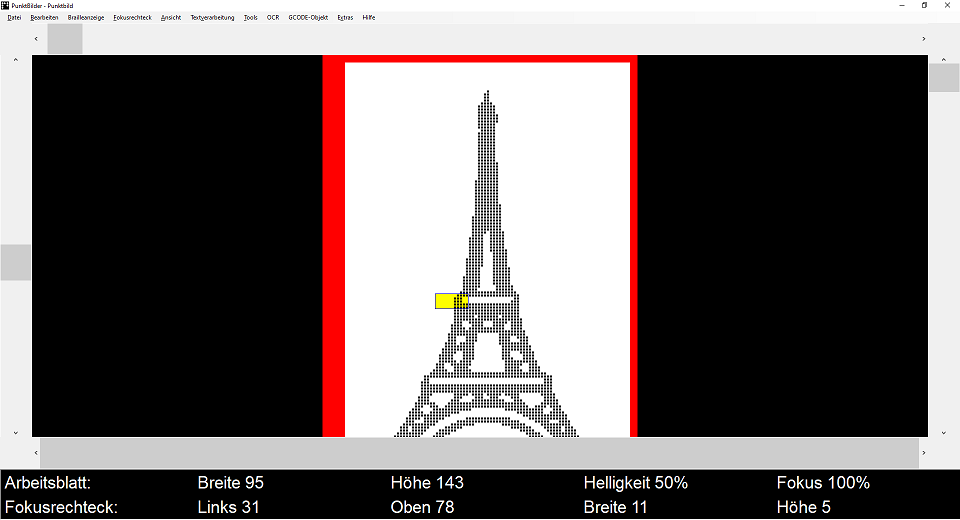
\includegraphics[width=0.7\linewidth]{img/PunktBilder.png}
    \caption{Screenshot from the \textit{PunktBilder} application (Source: THM / BliZ)}
    \label{fig:punktbilder}
\end{figure}

\begin{figure*}[ht!]
    \centering
    \begin{subfigure}[t]{0.5\textwidth}
        \centering
        
\includegraphics[width=.5\linewidth]{img/THM_Pattern.pdf}
      
    \end{subfigure}%
    \begin{subfigure}[t]{0.5\textwidth}
        \centering
        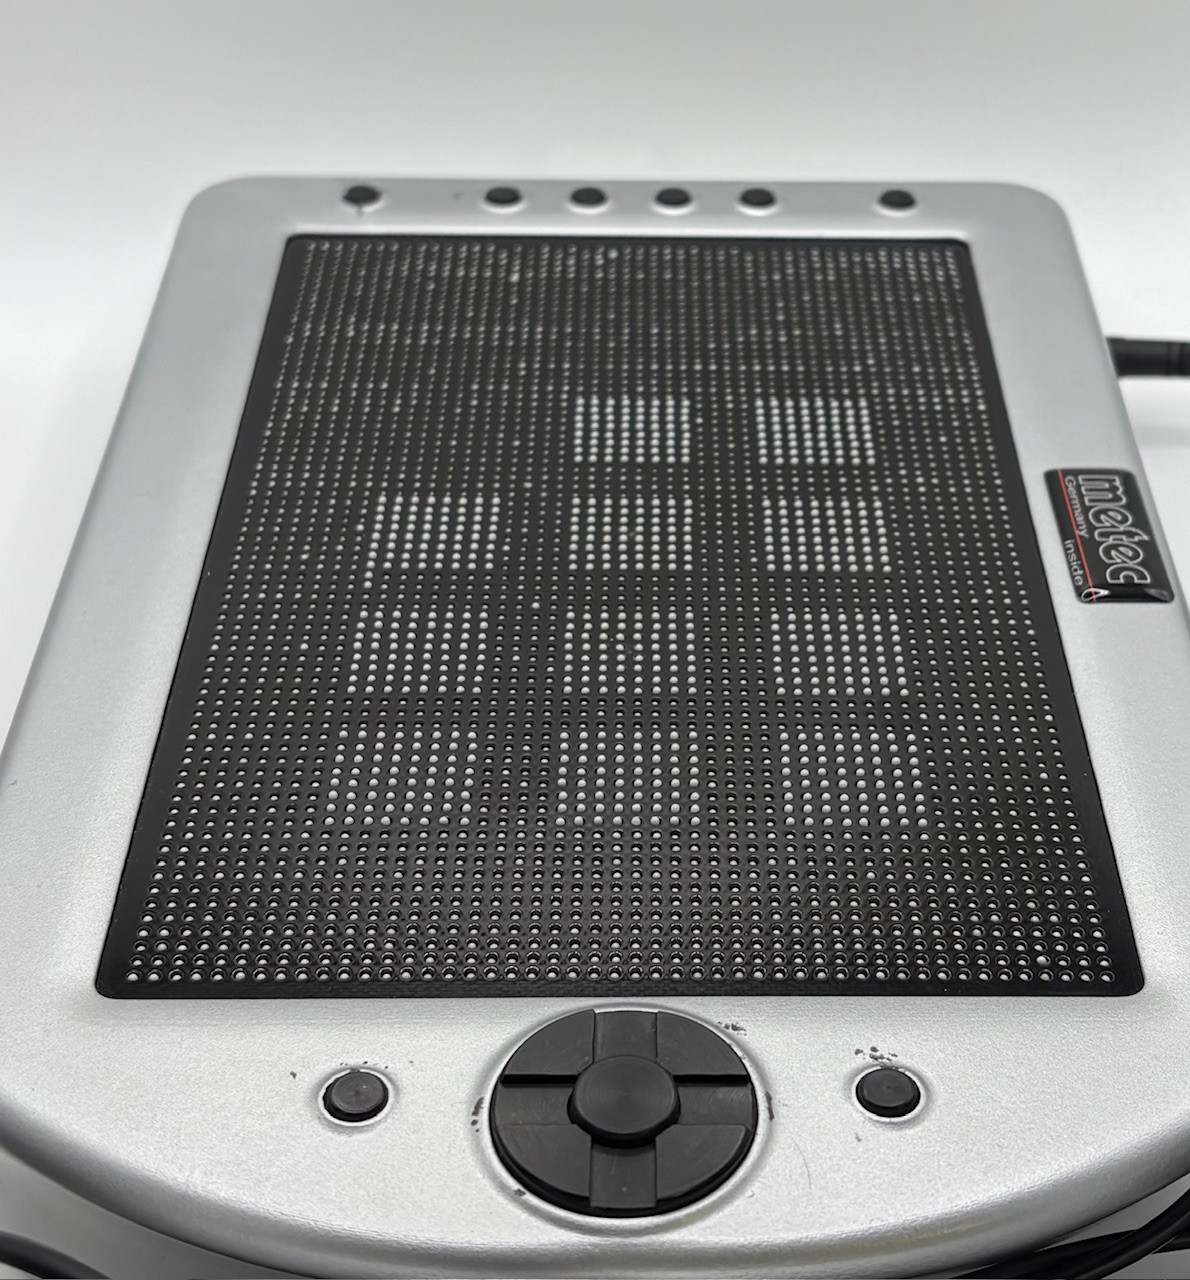
\includegraphics[width=.5\linewidth]{img/PunktBilder-BliZ.jpg}       
    \end{subfigure}
    \caption{Dot pattern for the logo of the THM (left), converted with \textit{PunktBilder} for a 2D Braille display (right) (Source: THM / BliZ)}
    \label{fig:punktbilder2}
\end{figure*}


\subsection*{Consequences}

% Benefits
\renewcommand{\labelenumi}{$+$}
\begin{enumerate}
\item Multi-modal accessibility is achieved by making textual explanations of graphics accessible using assistive technology. 

\item Generative AI can take over the creation of textual descriptions of graphics for authors.

\item The use of ‘alt text’ in HTML documents better fulfills regulatory requirements for accessibility. 


\end{enumerate}

% Liabilities
\renewcommand{\labelenumi}{$-$}
\begin{enumerate}
\item The manual creation of textual descriptions of graphics is time-consuming, and consideration must be given to which aspects and content of a graphic are significant.

\item The automatic generation of textual descriptions Generative AI should be checked by authors for content accuracy.

\item Devices for the production of tactile output formats such as 3D printers or thermal printers are expensive and complex to use.

\item Devices for dynamically changeable tactile outputs are expensive and require special software to control them. 
\end{enumerate}

 
\subsection*{Related Work}

Non-profit organizations like \textit{ProBlind}\footnote{\url{https://www.problind.org/en/}} are actively working to improve access to graphics for blind and visually impaired individuals. As part of a global community initiative, they are developing a free online database of tactile graphics, accessible worldwide. They have developed a tool chain to convert graphics into tactile graphics, as shown in Fig.~\ref{fig:problind}.

\begin{figure}[ht]
    \centering
    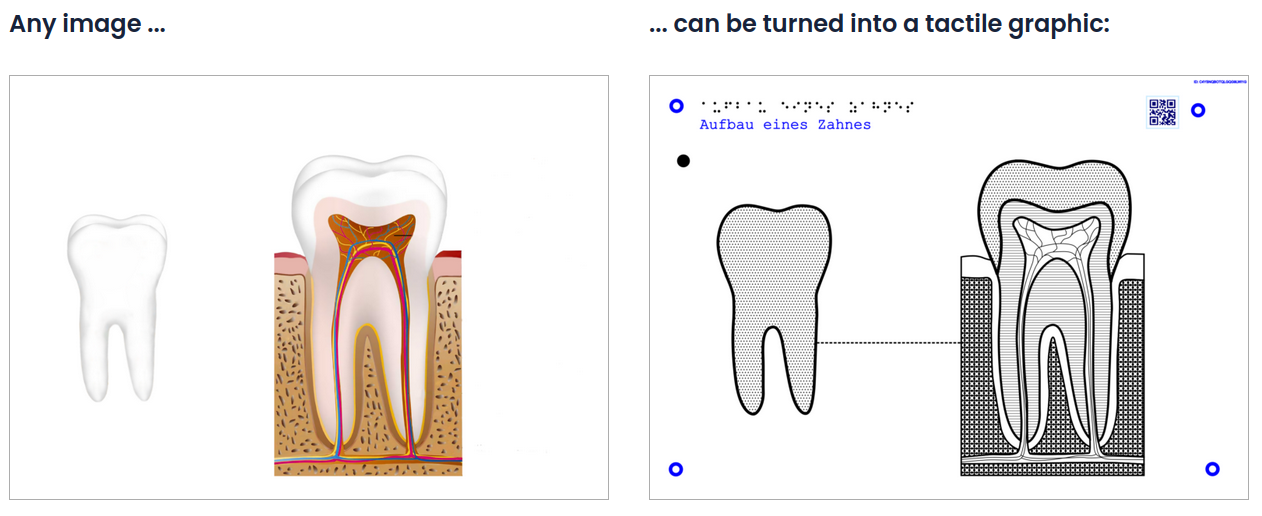
\includegraphics[width=.8\linewidth]{img/problind.png}
    \caption{Generation of tactile graphics (Screenshot from \texttt{www.problind.org})}
    \label{fig:problind}
\end{figure}

Many other schools for the blind and organizations that support the blind and visually impaired provide libraries of graphics that can be printed as tactile graphics.


In \cite{pissaloux2022} 
the accessibility challenges faced by visually impaired people  in interpreting graphical data, such as images and maps, is addressed. Their solution introduces the concept of a tactile gist as a simplified, touch-based representation of essential visual information. Based on experiments with VIP participants, the study establishes new design rules for 2D tactile representations using two mediums: thermo-formed paper and a force-feedback tablet called F2T.

In \cite{gay2021} this Force-Feedback Tablet (F2T) is introduced. The F2T’s architecture is based on a flat thumb-stick mounted on a 2D actuated support, enabling force feedback effects on user’s finger.


In \cite{ducasse2018} the challenge of accessibility of maps is addressed. The authors pointed out, that mobility and orientation are major challenges for visually impaired individuals. Primarily because verbal descriptions and GPS systems do not effectively convey spatial layouts. Unlike sighted individuals who rely on visual perception or maps, visually impaired people face limited access to geographical maps, which significantly impacts their mobility. The authors review various accessible interactive map solutions developed for visually impaired users, including a range of prototypes such as 3D-printed maps and devices with dynamically actuated structures.

%\patternFour

\subsection*{Context}

    Time series are widely used in science and engineering. Examples are the results of experiments, laboratory analyses or simulation results.
Such data is usually represented as a sequence of tuples (time | value). 
To analyze and interpret such results, they are displayed visually as graphs.
    
\subsection*{Problem}

\begin{itshape}

Graphical representations of time series  are not accessible for \ac{bvi} students and people in general. A sequential output of the data on Braille lines or by means of text-to-speech is not well suited to represent and convey the time based aspect of the data.   

\end{itshape}

\subsection*{Solution}


\begin{sol}

Provide sonifications of time series.
\end{sol}

Sonification is the use of non-speech audio to convey information.
For a time series  $x(t)$, data points can be mapped to sound parameters:
amplitude, rate of change, loudness or stereo position etc. 
\ac{bvi} students can listen as time unfolds, effectively hearing the trend.

Advanced sonification techniques comprise spatial audio (3D audio, auralization), where time or value is represented by left–right panning for added dimensionality.



\subsection*{Examples}

Highcharts\footnote{\url{https://www.highcharts.com/}}, in collaboration with the Sonification Lab at the Georgia Institute of Technology, has developed a free tool that enables the exploration of time series as charts and their sonification, employing sound as a medium for data visualization.

The charging of a capacitor is covered in \ac{stem}courses  for several reasons: it illustrates central concepts important in many disciplines, such as the creation of differential equations or the modeling and simulation of technical systems.

Fig.~\ref{fig:rc} shows a typical circuit for charging a capacitor via a resistor. The time constant $\tau$ is calculated from the product of the capacitance $C$ and the resistance value $R$: $\tau = R * C$.
The charging curve is described by the following formula: 


\[
U(t) = U_0 * (1- e^{-{ \frac{t}{\tau}}})
\]



\newpage
Listing \ref{lst:rc} shows the first 20 entries of a time series of charging a capacitor via a resistor($\delta t = 0.1$, $\tau = 2$).


\begin{lstlisting}[label=lst:rc, caption = time series of charging a capacitor]
t,U
0,0
0.1,0.48770575499286
0.2,0.951625819640405
0.3,1.39292023574942
0.4,1.81269246922018
0.5,2.21199216928595
0.6,2.59181779318282
0.7,2.95311910281287
0.8,3.29679953964361
0.9,3.62371848378227
1,3.93469340287367
1.1,4.23050189619513
1.2,4.51188363905974
1.3,4.77954223238984
1.4,5.03414696208591
1.5,5.27633447258985
1.6,5.50671035882778
1.7,5.72585068051273
1.8,5.93430340259401
\end{lstlisting}

This time series was imported and Highcharts generated the chart shown in Fig.~\ref{fig:sonification}. On top of the page, there are the buttons for playing the sound: Play, Stop and Loop.  

\begin{figure}
    \centering
    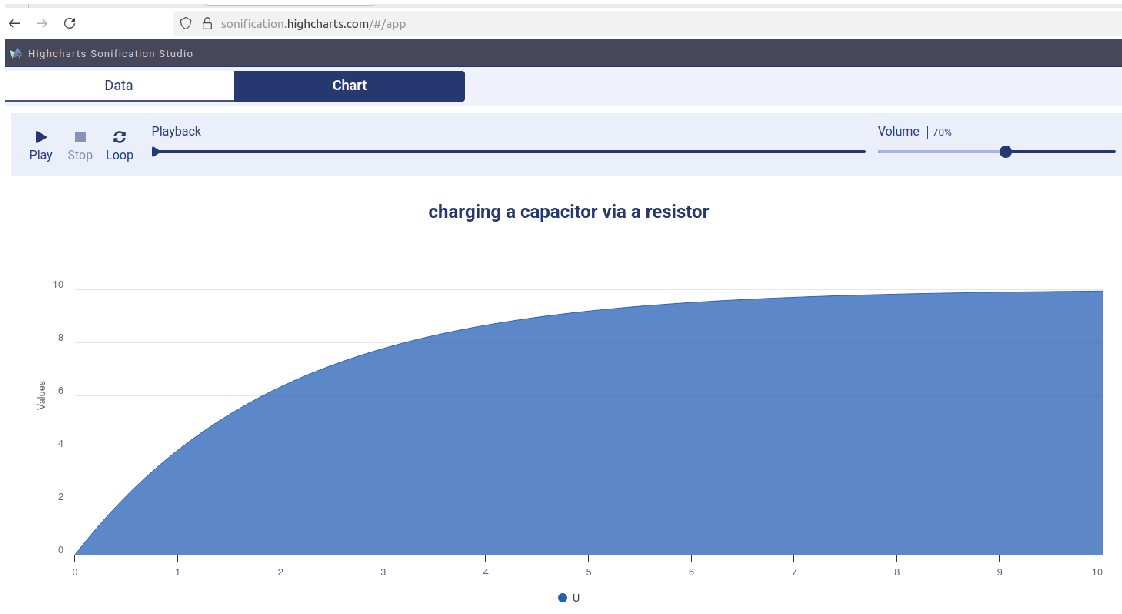
\includegraphics[width=\linewidth]{img/sonification.pdf}
    \caption{Screenshot from the sonification web site}
    \label{fig:sonification}
\end{figure}
 
\subsection*{Consequences}

% Benefits
\renewcommand{\labelenumi}{$+$}
\begin{enumerate}
\item Time series usually contain the temporal progression of signals; sonification allows the dimension of time to be experienced intuitively.

\item Some tools allow the playback speed to be adjusted or zoomed in on specific points in time.

\item Web-based solutions are easy to use for sonification and are usually easily accessible.

\end{enumerate}

% Liabilities
\renewcommand{\labelenumi}{$-$}
\begin{enumerate}
\item Understanding and correctly interpreting audible time series requires experience and training, among other things.

\item Devices for spatial audio reproduction are more expensive than normal headphones.

\item Sonification software usually needs to be installed, and training in the use of the software is necessary. 
\end{enumerate}
 
 
\subsection*{Related Work}

In \cite{potluri2022psst} Physical-computing Streaming Sensor data Toolkit (PSST) is introduced. This  toolkit enables \ac{bvi}  developers to create accessible representations of real-time sensor data. PSST allows users to filter, highlight, and transform time series of raw or computed sensor values into different output formats including tonal sonification, non-speech audio, speech, and SVG files for tactile displays. 

in \cite{casado2021} SonoUno is presented. It is a sonification software for astronomical data presented on a table (txt or csv files). Goal of the project is enabling accessibility to scientific data, from the Earth or with instruments on board of satellites. Such data is available in databases
such as Simbad, NASA, ESA, among others.

The study presented in \cite{Last2015} tested the hypothesis that musical sonification can serve as an effective alternative to visualizing time-series data when visual representation is unavailable or not accessible especially for \ac{bvi} people. The authors developed a time-series sonification method that can translate both uni-variate and multi-variate time series into a musical format.

In \cite{damsa2024}  a study examining the educational outcomes of \ac{bvi} children aged 0 to 8  learning  sonification concepts is presented. 
\ac{bvi} children  face significant barriers to participating in Science, Technology, Engineering, and Mathematics (STEM) education and careers, which have traditionally depended on visually based information. The authors had developed  an app „Sonoplanet“ for the sonification in an  educational context.


%\patternFive

\subsection*{Context}

Graphics are an important way of presenting information for sighted people.  
Images are frequently used in electronic media such as websites and online platforms. In teaching, images are often used in web-based materials to convey content. Other digital resources - such as lecture notes, exercise sheets and presentation slides - also tend to contain a variety of images, graphics and illustrations.
    
\subsection*{Problem}

\begin{itshape}
Although electronic media can be made accessible to blind and visually impaired users through the use of assistive technologies, this does not usually work for the graphic components embedded in these media. As a result, the information conveyed by visual representations often remains inaccessible to people with visual impairments.
\end{itshape}


\subsection*{Solution}


\begin{sol}

Augment visually represented information with a generated and verified textual description.

\end{sol}

In \ac{html} files the so called "alt text"  (alternative text) can give an additional text-based descriptions of visual details of an image. 
Originally this "alt text" is intended to give some information if the HTML page is not loaded properly. 
Such descriptions are useful to provide accessible information for people who are visually impaired. This approach can be applied to other formats, too.

Additional information about a graphic can be embedded as metadata. Assistive technologies such as 2D Braille displays can then present this information as text or text-to-speech tool can produce audio output.

Emerging artificial intelligence technologies are increasingly capable of interpreting and describing graphics. These advancements offer promising solutions for making visual content more accessible to blind and visually impaired individuals.



\subsection*{Examples}
 
Fig.~\ref{fig:freehand} illustrates the problem of mixing text which can be found by assisting tools within a picture. e.g., a text-to-speech tool will say "Dog" without a contextual relation.
A solution would be a picture in a pixel image format and additional the picture describing text. Artificial intelligence tools can generate such texts. Generated texts should be checked by the authors.
Fig.~\ref{fig:instantiation} shows a .png picture illustrating the concept of instantiation. The arrow follows the UML specification. 

\begin{figure}[ht]
    \centering
    \fbox{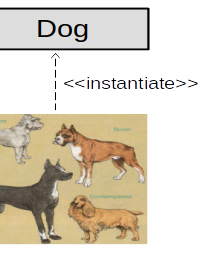
\includegraphics[width=0.5\linewidth]{img/instanziierung.png}}
    \caption{Visualization of the concept of instantiation in object-oriented programming}
    \label{fig:instantiation}
\end{figure}

Here a generated description of this picture (chatGPT):
\begin{quote}
This image is a visual metaphor for the \ac{oop} concept of instantiation.

Description:

- At the top of the image, there's a gray box labeled "Dog", which represents a class in OOP.

- Below it, there is a picture of different dog breeds (e.g., Boxer, Cocker Spaniel, etc.).

- A dashed arrow labeled <<instantiate>> points from the dog images to the class "Dog", indicating that these individual dogs are instances (objects) of the class.
\end{quote}

Simulation of electronic circuits is an important topic in technical electronics and technical informatics. Fig.~\ref{fig:rc} shows a screenshot of a circuit and a simulation result using the simulation tool LT-Spice.

\pagebreak

An AI-generated description of this figure can be improved if the context is given in the prompt: "explain this figure in the context of technical electronics"

\begin{figure}[ht]
    \centering
    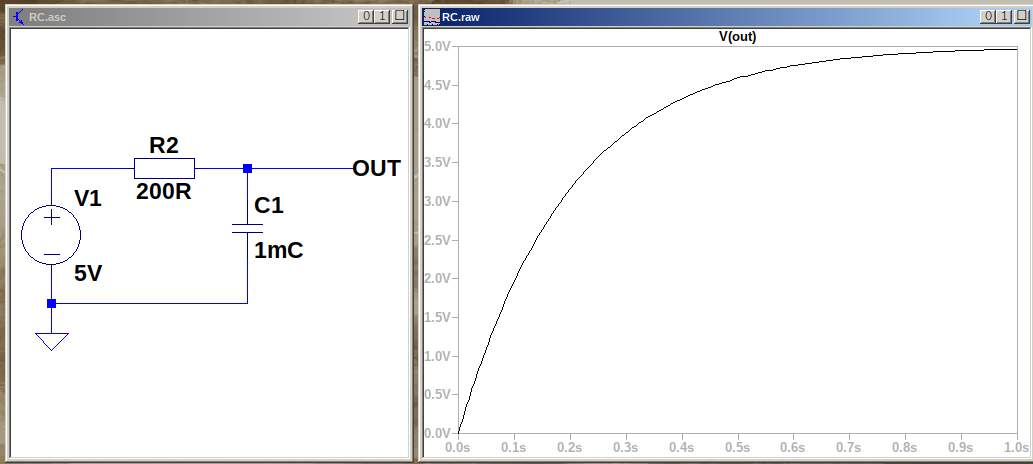
\includegraphics[width=0.9\linewidth]{img/RC.png}
    \caption{Screenshot of Circuit and Timeline Graph}
    \label{fig:rc}
\end{figure}


Answer from chatGPT:
\begin{quoted}
    

This figure illustrates the behavior of a simple RC (Resistor-Capacitor) charging circuit, commonly studied in technical electronics to understand transient response in linear time-invariant systems.

Left Side: Circuit Diagram

    The left side of the figure shows the schematic diagram of an RC circuit. It consists of:
\begin{itemize}
  \item A DC voltage source \( V_1 = 5\,\text{V} \)
  \item A resistor \( R_2 = 200\,\Omega \)
  \item A capacitor \( C_1 = 1\,\text{mF} \)
\end{itemize}

The resistor and capacitor are connected in series, and the voltage across the capacitor (marked as \texttt{OUT}) is observed over time. This configuration is typically used to study the charging process of a capacitor.

Right Side: Voltage-Time Plot

   The right side of the figure displays the simulation output: a voltage-time plot of \( V_{\text{out}} \), the voltage across the capacitor, from \( t = 0 \) to \( t = 1 \) second.

The voltage exhibits an exponential rise, which is characteristic of a capacitor charging through a resistor. The governing equation is:

\[
V(t) = V_{\text{source}} \cdot \left(1 - e^{-t/RC}\right)
\]

where:
\begin{itemize}
  \item \( V_{\text{source}} = 5\,\text{V} \)
  \item \( R = 200\,\Omega \)
  \item \( C = 1\,\text{mF} \)
  \item \( \tau = RC = 0.2\,\text{s} \) is the time constant
\end{itemize}

At approximately \( t = \tau \), the capacitor reaches about 63\% of its final value. The graph confirms that the capacitor voltage asymptotically approaches 5V, with the majority of charging occurring within the first second.

...

It serves as a fundamental demonstration of key concepts including time constants, exponential behavior, and transient analysis in electrical circuits.

\end{quoted}



\subsection*{Consequences}

% Benefits
\renewcommand{\labelenumi}{$+$}
\begin{enumerate}
\item The use of ‘alt text’ in HTML documents ensures that regulatory requirements for accessibility are better met. 

\item Generative AI can be used by authors to  create textual descriptions.

\item Generative AI tools can be integrated into your own applications. For example, a Python script can be used to add excellent "alt text" to entire folders full of images.


\item The generated explanation is not only helpful for blind and visually impaired people to gain access to the illustration. Sighted students can also benefit from this description.
\end{enumerate}

% Liabilities
\renewcommand{\labelenumi}{$-$}
\begin{enumerate}
\item Automatically generated descriptions should be checked by authors to ensure that the content is correct.
\end{enumerate}
 
\subsection*{Related Work}

The generation of explanatory text for graphics has been studied from both
automated and human-centered perspectives. Evaluations of automatic image
captioning systems show that while machine-generated descriptions can provide
basic accessibility, their quality often lacks accuracy and specificity,
highlighting the need for human editorial review
\cite{Leotta2023AutoCaptioning}. Complementary research on alternative text
creation documents the roles and processes through which authors, editors, and
reviewers collaboratively ensure reliable descriptions, emphasizing that
"alt text" production is a socio-technical practice rather than a purely
technical task \cite{Edwards2023AltTextProcess}. In addition, user studies with
blind and visually impaired participants underline that effective descriptions
must focus on data content, task relevance, and structural clarity rather than
only surface-level visual features \cite{Jung2021AltText}. Together, these
findings support our approach of combining automated captioning with
human-in-the-loop validation to ensure pedagogically useful and trustworthy
explanations of graphics.

% AI Tutor

\patternSix

\subsection*{Context}

\ac{bvi} students are increasingly represented in \ac{stem} degree programs. In these disciplines, instruction relies on visual learning materials such as lecture slides, scripts, exercise sheets, diagrams, circuit schematics, graphs, and tables. Although accessibility standards exist, many teaching materials remain only partially accessible or entirely inaccessible to students who depend on screen readers or text-based representations.


\subsection*{Problem}

Core teaching materials in \ac{stem} courses are frequently inaccessible to BVI students. In particular, graphical representations such as diagrams, plots, \ac{kv} maps, circuit schematics, and state machines cannot be consumed directly with screen readers.

Students may use general-purpose AI systems (e.g., ChatGPT) to obtain text-based explanations or descriptions of visual content. However, this ad hoc approach requires repeated prompting and reintroducing course context for each document. The accessibility burden is shifted to the student, leading to unequal learning conditions and avoidable inefficiencies.


\subsection*{Forces}
\renewcommand*\labelitemi{\textbullet}
\begin{itemize}
    \item \ac{stem} education relies heavily on visual abstractions.
    \item Teaching staff often lack time or expertise to fully redesign materials for accessibility.
    \item \ac{bvi} students need structured, consistent, and context-aware explanations.
    \item General-purpose AI tools are powerful but lack course-specific knowledge unless carefully prompted.
    \item Accessibility solutions must scale across courses without excessive manual effort.
\end{itemize}

\subsection*{Solution}

\begin{sol}
Configure a course-specific, \ac{llm}-based AI tutor grounded in the materials, terminology, and learning objectives of a particular course, and enforce explicit accessibility rules for \ac{bvi} students. A Custom GPT is one practical implementation of this idea.
\end{sol}

To resolve the challenges of visual reliance in \ac{stem},  limited instructor time,  the need for consistent, context-aware explanations, and scalability across semesters, the tutor is set up as a reusable and maintainable resource with three building blocks:

\begin{itemize}
    \item Instruction policy
    \newline
    Define a stable interaction and accessibility policy: the AI tutor has to explain content in a linear and screen-reader-friendly language. Avoid purely spatial references like ``left/right/top/bottom'' and purely decorative elements like emojis (see Pattern 1 \textsc{Core of Content}). 
    

    \item Curated course knowledge base
    \newline
    Provide course documents as the primary reference (lecture slides, script, exercise sheets, learning goals) and add compact guideline documents that encode recurring conventions. In our case these include (i) an accessibility guideline (how to describe figures, \ac{kv} maps, and time series) and (ii) a CircuitJS-to-SPICE mapping with examples and templates. This supports scalability and reduces repeated manual explanations.

    \item Well defined transformation workflows
    \newline
    Establish repeatable workflows for typical artifacts:
    \begin{enumerate}
        \item \emph{PDFs, slides or figures}: (1) short overview, (2) structured description of elements and connections, (3) interpretation of meaning/function in the course context.
        \item \emph{Electronic Circuits}: (1) verbal reconstruction of the schematic (nodes, components, polarity), (2) generation of a commented SPICE/LTspice netlist using speaking node names, (3) explicit marking of assumptions if the source is ambiguous.
        \item \emph{Simulation output}: prefer text-first result reporting e.g. as  tables  over graphical plotting, such that \ac{bvi} students can inspect results with screen readers.  Pattern 3 \textsc{Accessibility of Graphics} introduces solutions for accessing plottings and Pattern 4 \textsc{Sonification of Time Series} 
shows a solution for making tabular time series, which are a typical textual outputs of simulation programes, accessible via the ear as an alternative channel.  
    \end{enumerate}
\end{itemize}

To support adoption and quality assurance, provide two short documents alongside the tutor:
\begin{itemize}
    \item An \textit{instructor manual} describing how to prepare materials for the knowledge base (consistent naming, missing figure descriptions, update workflow), and
    \item An \textit{accessible student guide} describing how to upload documents, request different levels of explanation, and ask for conversions, e.g. ``describe the circuit and the simulation result''.
\end{itemize}

Finally, maintain the AI tutor through a lightweight quality assurance process:  run a small set of standard test prompts like the generation of figure descriptions whenever new materials are added. Adjust the instruction policy and guideline documents if recurring failure modes appear.

\subsection*{Resulting Context}

Students gain access to a persistent, course-aware AI tutor that can explain lecture content, exercises, and graphical representations in an accessible, text-based form. The individual effort required to make materials accessible is significantly reduced.

Instructors are supported rather than burdened, as they do not need to manually create alternative materials for every student. The approach improves inclusivity while preserving the original structure and learning objectives of the course.

\subsection*{Examples}

The pattern was applied in the course ``Technical Informatics~1 (TI-1)'' at a university of applied sciences. A dedicated tutor instance was provided to students (e.g., via a course link such as \url{https://chatgpt.com/g/g-691ee1833a4481919e30b6c052201050-technische-informatik-1-tutor-fur-blinde}). The following examples illustrate typical usage scenarios.

\begin{enumerate}
    \item Conversion of exercise sheets into  linear, screen-reader-friendly tasks.\\
    \emph{Input:} A student uploads a PDF exercise sheet with multi-column layout and embedded figures.\\
    \emph{Request:} ``Summarize the sheet, then rewrite all tasks in a linear format for a screen reader. Replace \ac{kv} map figures with minterm lists and provide a text table for any plotted signals.''\\
    \emph{Output:} The tutor produces (i) a short overview of the sheet, (ii) a numbered, linear task list without layout dependencies, and (iii) textual substitutes for visual elements (e.g., minterm/maxterm lists, truth tables in text form, and time/value tables for signals).

    \item Generation of figure and diagram explanations with progressive disclosure.\\
    \emph{Input:} A lecture slide containing a diagram (e.g., Wheatstone bridge, timing diagram, or block diagram).\\
    \emph{Request:} ``Describe the figure in two sentences first, then give a structured description of all elements and connections. Finally, explain what the diagram means in the context of this lecture.''\\
    \emph{Output:} The tutor follows the defined workflow: short overview, structured description (components/nodes/relations), and an interpretation that links the figure to course concepts. Students can then ask follow-up questions to increase or decrease the level of detail.

    \item Conversion of CircuitJS schematics into commented SPICE/LTspice netlist with accessible results.\\
    \emph{Input:} A CircuitJS screenshot or exported text of a circuit used in an assignment (e.g., diode rectifier, transistor inverter, RLC transient).\\
    \emph{Request:} ``First describe the circuit in words (nodes, components, polarity). Then generate a commented LTspice netlist using speaking node names. Include text-first output using \texttt{.print} and key metrics with \texttt{.measure} in the simulation tool. Mark any assumptions explicitly.''\\
    \emph{Output:} The tutor returns (i) a verbal reconstruction, (ii) a commented netlist suitable for screen readers, and (iii) an accessible evaluation setup (tables and measurements) enabling \ac{bvi} students to inspect simulation results without graphical plotting.
\end{enumerate}

\subsection*{Consequences}

\noindent\textbf{Benefits}
\begin{itemize}
    \item[$+$] Visual course artifacts like figure, schematics, \ac{kv} maps, and timing diagrams become available as linear, screen-reader-friendly explanations.
    \item[$+$]  Students no longer need to repeatedly convert course content by their own. The AI tutor follows a stable instruction policy, which results in accessible learning material of better quality.
    \item[$+$] By preferring text-first outputs  over graphical plotting, simulation results become accessible using screen readers or Braille displays.
    \item[$+$]  Once the AI tutor is configured correctly for the generation of accessible course material, incremental updates can be done with less effort when new sheets/slides are added.
    \item[$+$] The generated accessible learning materials provide an increased independence and alternative ways of self-paced learning.
\end{itemize}

\noindent\textbf{Liabilities}
\begin{itemize}
    \item[$-$] The quality of the generated accessible learning materials  depends on input quality and curation. Inconsistent terminology, missing figure context, or outdated materials reduce explanation quality. An ongoing maintenance of the knowledge base is required.
    \item[$-$] Using AI tools come along withe the risk of inaccuracies and hallucinations. Misread or ambiguous figures may lead to incorrect explanations. Human verification of the material is required, which is an additional effort.
    \item[$-$] Creating the instruction policy, guideline documents, and short instructor/student manuals requires initial effort before benefits materialize.
    \item[$-$]  AI tutors can improve consistency but  become outdated if changes in exercises, notation, or tools are not processed in time.
    \item[$-$] Without careful framing, students may over-rely on the AI tutor. Instructors should define recommended or acceptable use of the AI tutor and consider privacy/copyright constraints for uploaded materials.
\end{itemize}

\begin{comment}
   

\subsection*{Related Patterns}

\begin{itemize}
    \item \textbf{Accessible by Design:} Designing teaching materials and tools with accessibility as a first-class concern rather than as an afterthought is a core principle of inclusive education and universal design \cite{w3c2023,burgstahler2015}. The AI tutor pattern complements this approach by enabling accessibility even when legacy materials are not fully accessible.
    \item \textbf{Human-in-the-Loop Accessibility:} Instructors remain responsible for structuring and contextualizing materials, while the AI performs repetitive transformation and explanation tasks. This aligns with human-centered and human-in-the-loop AI concepts, where automation supports but does not replace human expertise \cite{shneiderman2020,ieee2019}.
    \item \textbf{Personal Learning Tutor:} The AI tutor acts as an individualized learning assistant that adapts explanations to the learner’s pace and prior knowledge. Such adaptive tutoring systems are a well-established application area of AI in education \cite{holmes2019}.
    \item \textbf{Progressive Disclosure of Complexity:} Students can request explanations at different levels of detail, supporting incremental learning and multiple representations of knowledge, which are central principles of Universal Design for Learning \cite{burgstahler2015,al-azawei2016}.
    \item \textbf{Single Source of Truth:} Teaching materials remain unchanged for the general audience while accessibility is generated dynamically through the AI. This reduces parallel document maintenance and supports sustainable accessibility practices \cite{lazar2015}.
\end{itemize}


\subsection*{Known Uses}

\begin{itemize}
    \item \textbf{Technical Informatics~1 (course-specific AI tutor).}
    The pattern has been applied in the course ``Technical Informatics~1 (TI-1)'' at a university of applied sciences. Students were provided with a dedicated tutor instance (e.g., via a course link such as \url{https://chatgpt.com/g/g-691ee1833a4481919e30b6c052201050-technische-informatik-1-tutor-fur-blinde}) to obtain linear, screen-reader-friendly explanations of lecture and exercise materials. Typical use included (i) rewriting exercise sheets into a linear format, (ii) structured descriptions of figures and diagrams, (iii) conversion of CircuitJS schematics/exports into commented SPICE/Ngspice netlists, and (iv) interpretation of simulation results via text-first outputs (e.g., \texttt{.print}/\texttt{.measure}) rather than graphical plots.

    \item \textbf{Informal use of general-purpose (multimodal) AI as an accessibility aid.}
    Beyond course-specific deployments, blind and visually impaired learners increasingly use general-purpose AI systems to obtain descriptions of visual content and to translate diagrams into natural-language explanations. Recent evaluations of multimodal LLMs as visual assistants document both the potential of such tools and the need for reliability safeguards, error handling, and uncertainty communication \cite{Karamolegkou2025}.

    \item \textbf{LLM-based interaction for accessible visual artifacts (charts/diagrams).}
    Related pilot systems and studies show how conversational interaction can improve accessibility of visual artifacts such as charts and diagrams, supporting exploration through structured responses instead of purely visual inspection \cite{Gorniak2024VizAbility,Sharif2025VoxEx}. These uses align with our pattern by treating LLMs as a mediation layer that turns visual encodings into accessible representations.
\end{itemize}

Although still emerging, these uses indicate that LLM-based tutoring can act as an accessibility amplifier in higher education when embedded within responsible, human-centered design and maintenance practices \cite{shneiderman2020,ieee2019,lazar2015}.
\end{comment}

\newpage
\subsection*{Related Work}

Recent work explores \ac{llm} and \ac{mllm} based tools as assistive technologies that translate visually encoded information into representations that can be perceived and navigated by \ac{bvi} users. Empirical evaluations indicate that \ac{mllm}s can support common visual assistance tasks, while reliability and error handling remain central challenges for broader use \cite{Karamolegkou2025}. 

In the domain of data visualizations, conversational systems such as \textit{VizAbility} demonstrate how dialogue-based interaction can augment chart exploration \cite{Gorniak2024VizAbility}. Complementary work emphasizes that accessibility is not achieved by static descriptions alone but depends on interaction mechanisms that preserve user agency and enable independent exploration with screen readers \cite{Sharif2025VoxEx}. %Pattern~6 transfers these insights to \ac{stem} course materials and simulation results by prioritizing text-first outputs and structured explanations over purely graphical representations.

A second line of related research focuses on making diagram semantics explicit so that users can query or learn from diagrams through language-based interaction. Approaches that generate detailed textual descriptions of diagrams for \ac{llm}-based exploration illustrate how ``silent'' graphics can be bridged into structured natural language, supporting accessible learning pathways for \ac{bvi} users \cite{Wegwerth2023Diagram}. 

There is ongoing research how to extract circuit structure from schematics and generating netlists automatically. \cite{Hemker2024Schematics,Huang2025Netlistify} present deep-learning-based schematic-to-netlist pipelines demonstrating progress in component recognition and connectivity extraction. 

For time-dependent simulation outputs, related state-of-the-art work on sonification (see Pattern 4 \textsc{Sonification of Time Series}). Haptic feedback gives an additional non-visual access that can complement text-based traces and key metrics \cite{Spagnuolo2025Sonification}.


\patternSeven

\subsection*{Context}

\ac{bvi} students are increasingly represented in \ac{stem} (Science, Technology, Engineering, and Mathematics) degree programs. In computer science and engineering courses, learning is often driven by large collections of written materials such as lecture scripts, slide decks, exercise sheets, lab instructions, and reading assignments. \ac{bvi} students typically consume these materials through screen readers or Braille displays, which provide linear access; navigating and revisiting long documents is time-consuming.

Some students also benefit from alternative representations when sustained reading is challenging (e.g., dyslexia) or because initiating and sustaining attention on long texts is difficult (e.g., \ac{adhd}). For some autistic students, predictable structure and reduced cognitive overload can be beneficial, while others may prefer text over audio. These groups are secondary beneficiaries of this pattern; the primary accessibility motivation and constraints focus on \ac{bvi} learners.

This pattern applies both the teaching contexts with bundles of course materials and, with similar constraints, to academic work for a first-pass reading of long papers or book chapters.

\subsection*{Problem}

Long documents and heterogeneous material collections are costly to consume and revisit when access is primarily linear using screen readers or Braille displays. Students may lose time and context, enter topics late, and struggle to prepare for tutorials and discussions.

Students can use general-purpose AI systems to create summaries as easier accessible versions of documents. However, this ad-hoc approach requires repeated context building and prompt engineering for each new document and week. The accessibility workload is shifted to the student and does not scale.

In \ac{stem}, materials often include diagrams, plots, and schematics that are not inherently accessible. AI generated descriptions can support semantic orientation, but they do not replace precise accessible representations of visual artifacts.


\subsection*{Forces}
\renewcommand*\labelitemi{\textbullet}

\begin{itemize}
    \item Audio summaries are useful, but may contain omissions or inaccuracies. Quality assurance of the generated audios may become an additional effort.
    \item The audio should condense and restructure what is in the sources, but should not introduce novel aspects or even invented details.
    \item Some learners find audio distracting or unsuitable, hence alternatives must remain available.
    \item Pure audio is hard to skim. \ac{bvi} learners need additional information about the structure of documents like which chapter or timecodes. Ideally audio files are accompanied with  transcripts.
    \item Summaries must support learning without becoming a shortcut that replaces engagement with primary sources.
    \item Output quality depends on machine-readable, well-structured sources, but e.g. scan-only PDFs do not provide structural information.
    %\item Course materials and student submissions may be protected; institutional policies may restrict uploads or redistribution.
\end{itemize}

\begin{comment}
\begin{itemize}
    \item \textbf{Accuracy vs.\ effort:} Audio summaries are useful but may contain omissions or inaccuracies; quality assurance must not become a new large burden.
    \item \textbf{Faithfulness to sources:} The audio should condense and restructure what is in the sources, not introduce novel claims or invented details.
    \item \textbf{Audio helps many, not all:} Some learners find audio distracting or unsuitable; alternatives must remain available.
    \item \textbf{Navigability:} Pure audio is hard to skim; BVI learners need structure (chapters/timecodes) and ideally a transcript.
    \item \textbf{Assessment integrity:} Summaries must support learning without becoming a shortcut that replaces engagement with primary sources.
    \item \textbf{Source quality:} Output quality depends on machine-readable, well-structured sources (no scan-only PDFs; code should be text, not screenshots).
    \item \textbf{Privacy/IP constraints:} Course materials and student submissions may be protected; institutional policies may restrict uploads or redistribution.
\end{itemize}
\end{comment}
\subsection*{Solution}

\begin{sol}
Use a customized \ac{llm} tool specialized on generating overviews based on uploaded documents. 
Use the the audio overview feature of such tools to generate podcast-like, speech-first audio summaries from a curated bundle of course sources.
\end{sol}

Design the output to be speech-first, accessible, and faithful:
\begin{itemize}
    \item Start with learning objectives and a short overview.
    \item Define key terms and notation consistently.
    \item Provide  mini examples that illustrate the course style.
    \item Highlight common misconceptions.
    \item End with a short checklist (``You should be able to\ldots'') and ``what to read/do next.''
    \item Explicitly mark uncertainty and avoid adding details not supported by the provided sources.
\end{itemize}

Publish the audio as an  learning aid accompanied by additional information, especially a textual transcript and a chapter list with timecodes.
The audio is a learning aid and may contain errors or omissions, which should be declared in disclaimer.
%; primary sources remain authoritative.

Use different granularity levels to fit different needs, e.g., a short weekly overview, a longer deep dive for complex topics, and an exam-revision overview.

\subsection*{Resulting Context}

Instructors provide a reusable, low-friction first pass overview of course materials that reduces navigation overhead for \ac{bvi} students and supports preparation for tutorials and discussions. Students gain an additional channels, audio and transcript, that can be consumed flexibly  without replacing the original sources.

\subsection*{Examples}

The pattern was applied in the course ``Technical Informatics~1 (TI-1)'' at our university of applied sciences as a weekly pipeline: instructors curated a compact source bundle, generated an audio overview, and published audio, transcript and timecodes in the learning management system (LMS). In this case the used AI tool was NotebookLM\footnote{\url{https://notebooklm.google/}}. 

\begin{enumerate}
    \item Boolean operations and truth tables\\
    \emph{Input:} Text-first course content (e.g., Markdown-based core content rendered into slides) + and weekly exercise sheets.\\
    \emph{Request:} ``Create an Audio Overview with: (1) learning objectives, (2) key terms/notation, (3) one mini example, (4) two common misconceptions, (5) a checklist and next steps. Be faithful to the sources; mark uncertainty; avoid spatial references.''\\
    \emph{Output:} An audio overview, a transcript and chapter lists with timecodes covering AND/OR/NOT, truth-table construction, typical precedence pitfalls, and a short practice checklist.

    \item \ac{kv} maps \\
    \emph{Input:} Text-first KV-map representation generated from the exercise sheet.\\
    \emph{Request:} Same template, with emphasis on step-by-step strategy (grouping logic, minimization goals) and typical mistakes.\\
    \emph{Output:} Audio overview that provides intuition and a workflow for solving tasks. Audio output supports semantic orientation but does not replace a precise accessible KV-map representation.

    \item Circuit simulation interpretation\\
    \emph{Input:} Text-first simulation outputs tables of measured values with short additional explanations.\\
    \emph{Request:} Focus on interpretation: what metrics mean, how to compare cases, and how results link back to assumptions.\\
    \emph{Output:} Audio files and textual transcripts explaining which quantities matter, how to interpret changes, and a short checklist for reporting results.
\end{enumerate}

\subsection*{Consequences}

\noindent\textbf{Benefits}
\begin{itemize}
    \item[$+$] Podcast-Like audio summaries can provide a faster orientation over large material bundles. They reduce navigation overhead and support preparation for tutorials and discussions.
    \item[$+$]  Audio accompanied with textual information like a transcript and chapter list can be consumed flexibly and supports independent learning.
    \item[$+$] Students with dyslexia/ADHD benefit from a reduced reading load and lower entry barriers.
    %\item[$+$] \textbf{Scales for instructors.} A repeatable weekly pipeline yields consistent outputs with limited additional effort.
\end{itemize}

\noindent\textbf{Liabilities}
\begin{itemize}
    \item[$-$] AI generated materials may have inaccuracies and or e.g. misleading summaries. Quality assurance means an additional effort. Disclaimers should be added.
    \item[$-$] Important details of the original materials may be omitted due to condensation. Students have to consult primary sources for full fidelity.
    \item[$-$] Students may substitute audio summaries for primary sources, especially near assessments. Hence they may miss important details of the original course materials.
    \item[$-$] Audio can be distracting or unsuitable for some learners. Transcripts and text materials must remain available.
    \item[$-$]  Institutional policies may restrict what can be uploaded or redistributed.
\end{itemize}

\begin{comment}
\subsection*{Related Patterns}

\textbf{Pattern 6 (AI Tutor):} Use a course-specific, source-grounded tutor for precise transformations and explanations of visual artifacts (diagrams, schematics, KV maps). Pattern~7 complements this by providing orientation and revision via structured audio overviews.

\subsection*{Known Uses}
\begin{itemize}
    \item Applied in \textbf{Technical Informatics~1} as a weekly pipeline: instructors curate a short source bundle (script + accessible slide export + exercises), generate an Audio Overview, and publish audio + transcript + timecodes in the LMS.
    \item Used as a \textbf{first pass} before tutorials and as a \textbf{revision resource} during exam preparation.
\end{itemize}
\end{comment}

\subsection*{Related Work}

Structured educational podcasts have been studied as an accessible learning modality for \ac{bvi} users, showing that clear structure and navigability matter \cite{Buzzi2011StructuredPodcasts}. Speech-first summarization research emphasizes that summaries optimized for spoken output require different design choices than text summaries and should explicitly support linear comprehension \cite{McKeown2005TextToSpeech}. Recent accessibility research explores AI-assisted navigation and question answering to help \ac{bvi} learners access lecture content more efficiently \cite{Anderer2025LectureVideos}, aligning with our goal of reducing first-pass overhead for large material bundles. Recent studies of AI-generated educational podcasts report positive learner experiences and measurable learning outcomes in educational settings \cite{Do2024PAIGE}. 
Podcast-like course materials should be supplemented with textual information to enable targeted access to the audio information and to provide alternative channels.

%%% MK: Vorschlag
\section{Conclusion and Future Work}
\begin{comment}
This pattern collection presents simple solutions that make it easier for blind and visually impaired people to access graphically represented technical content with little effort. 

%The solutions were is paper has presented and empirically evaluated collection of patterns designed to make graphical representations in computer science and technical informatics education accessible to blind and visually impaired students.

The proposed solutions -- PlantUML or YAML formats for UML class diagrams, simplified LTspice netlists for electronic circuits, Java-based templates for logic circuits, and structured Markdown for \ac{kv} maps -- were derived from four years of practical experience with blind students in programming and technical informatics courses.

Structured interviews confirmed that these approaches are comprehensible, practical, and pedagogically effective, significantly lowering accessibility barriers and fostering inclusion in mixed-ability classrooms. Notably, the extracted textual content has proven valuable not only to visually impaired learners but also to sighted students, who appreciate the concise and well-structured representations. Our approach helps to create easy accessible course content using open source tools, ensuring equitable participation for blind, visually impaired, and sighted students alike.

Building on this foundation, future work will explore the integration of generative artificial intelligence (AI) to further enhance accessibility.
Our current work includes the automated generation of textual descriptions for graphical content and the creation of audio podcasts from course materials and textbooks to enable multi-modal access for a broader range of learners.

Generative AI for accessible content production has recently gained significant attention as a promising strategy for reducing educational barriers.
Research demonstrates that large language models and image-to-text systems can automatically generate alternative text, audio descriptions, or multi-modal summaries, thereby supporting blind and visually impaired learners in \ac{stem}  and other fields \cite{Karamolegkou2025}, \cite{Schauer2025}.

Upcoming research will therefore expand the existing pattern collection with new solutions leveraging AI-driven methods, investigate hybrid approaches that combine text-based formats with haptic or auditory feedback. Findings will be used to extend this pattern collection.
\end{comment}


Generative artificial intelligence has emerged as a promising approach to improving the accessibility of educational content and reducing barriers in higher education. Recent research indicates that large language models and image-to-text systems can support the automated generation of alternative text, audio descriptions, and multimodal summaries, thereby enhancing access to learning materials for \ac{bvi} learners in \ac{stem}  and related disciplines \cite{Karamolegkou2025,Schauer2025}. These developments highlight the potential of AI-assisted content creation as a scalable complement to established accessibility practices.

Building on these insights, future work will extend the existing pattern collection with solutions that incorporate AI-driven methods for accessible content production. In addition, we will explore hybrid approaches that combine text-based representations with haptic or auditory feedback to address diverse accessibility needs. The results will be systematically evaluated and used to further refine and expand the proposed pattern collection.

\subsection*{Acknowledgements} 



%\section{Related Patterns}
TODO:

Maybe these are candidates for new patterns

\begin{itemize}
    \item \textbf{Accessible by Design:} Designing teaching materials and tools with accessibility as a first-class concern rather than as an afterthought is a core principle of inclusive education and universal design \cite{w3c2023,burgstahler2015}. The AI tutor pattern complements this approach by enabling accessibility even when legacy materials are not fully accessible.
    \item \textbf{Human-in-the-Loop Accessibility:} Instructors remain responsible for structuring and contextualizing materials, while the AI performs repetitive transformation and explanation tasks. This aligns with human-centered and human-in-the-loop AI concepts, where automation supports but does not replace human expertise \cite{shneiderman2020,ieee2019}.
    \item \textbf{Personal Learning Tutor:} The AI tutor acts as an individualized learning assistant that adapts explanations to the learner’s pace and prior knowledge. Such adaptive tutoring systems are a well-established application area of AI in education \cite{holmes2019}.
    \item \textbf{Progressive Disclosure of Complexity:} Students can request explanations at different levels of detail, supporting incremental learning and multiple representations of knowledge, which are central principles of Universal Design for Learning \cite{burgstahler2015,al-azawei2016}.
    \item \textbf{Single Source of Truth:} Teaching materials remain unchanged for the general audience while accessibility is generated dynamically through the AI. This reduces parallel document maintenance and supports sustainable accessibility practices \cite{lazar2015}.
\end{itemize}
 % Ideensammlung / Pattern Candidates




\subsection*{Acronyms} 
\begin{acronym}[WYSIWYG]



\acro{ai}[AI]{artificial intelligence}

\acro{adhd}[ADHD]{attention-deficit/hyperactivity disorder}

\acro{csv}[CSV]{comma-separated values}

\acro{esa}[ESA]{European Space Agency}

\acro{gpt}[GPT]{generative pretrained transformer}

\acro{llm}[LLM]{large language model}

\acro{lms}[LMS]{learning management system}

\acro{mllm}[MLLM]{multimodal large language model}

\acro{nasa}[NASA]{National Aeronautics and Space Administration}

\acro{pdf}[PDF]{portable document format}

\acro{svg}[SVG]{Scalable Vector Graphics}

\acro{wai}[WAI]{Web Accessibility Initiative}

\acro{wcag}[WCAG]{Web Content Accessibility Guidelines}

\acro{bvi}[BVI]{blind and visually impaired }


\acro{gai}[GenAI]{generative artificial intelligence}

\acro{mds}[MDS]{Multimodal Diagrammatic System }

\acro{html}[HTML]{Hypertext Markup Language}


\acro{kv}[KV]{Karnaugh–Veitch}

\acro{mit}[MIT]{Massachusetts Institute of Technology}

\acro{oop}[OOP]{Object-Oriented Programming}

\acro{spice}[SPICE]{Simulation Program with Integrated Circuit Emphasis}

\acro{stem}[STEM]{Science, Technology, Engineering, and Mathematics}


\acro{tml}[TML]{textual modeling language}

\acro{uml}[UML]{Unified Modeling Language}

\acro{uncrpd}[UN-CRPD]{
United Nations Convention on the Rights of Persons with Disabilities}



\acro{who}[WHO]{World Health Organization}

\acro{wysiwyg}[WYSIWYG]{What You See Is What You Get}

\acro{xml}[XML]{Extensible Markup Language}
\acro{xmi}[XMI]{XML Metadata Interchange}

\acro{yaml}[YAML]{Yet Another Markup Language}

\end{acronym}

%
% ---- Bibliography ----
%
% BibTeX users should specify bibliography style 'splncs04'.
% References will then be sorted and formatted in the correct style.
%

 \bibliographystyle{splncs04}
  
 \bibliography{literature}

\end{document}

